%%%%%%%%%%%%%%%%%%%%%%%%%%%%%%%%%%%%%%%%%%%%%%%%%%%%%%%%%%%%%%%%%%%%%%
%%  Copyright by Wenliang Du.                                       %%
%%  This work is licensed under the Creative Commons                %%
%%  Attribution-NonCommercial-ShareAlike 4.0 International License. %%
%%  To view a copy of this license, visit                           %%
%%  http://creativecommons.org/licenses/by-nc-sa/4.0/.              %%
%%%%%%%%%%%%%%%%%%%%%%%%%%%%%%%%%%%%%%%%%%%%%%%%%%%%%%%%%%%%%%%%%%%%%%

\newcommand{\commonfolder}{../../common-files}

\documentclass[11pt]{article}

\usepackage[most]{tcolorbox}
\usepackage{times}
\usepackage{epsf}
\usepackage{epsfig}
\usepackage{amsmath, alltt, amssymb, xspace}
\usepackage{wrapfig}
\usepackage{fancyhdr}
\usepackage{url}
\usepackage{verbatim}
\usepackage{fancyvrb}
\usepackage{adjustbox}
\usepackage{listings}
\usepackage{color}
\usepackage{subfigure}
\usepackage{cite}
\usepackage{sidecap}
\usepackage{pifont}
\usepackage{mdframed}
\usepackage{textcomp}
\usepackage{enumitem}


% Horizontal alignment
\topmargin      -0.50in  % distance to headers
\oddsidemargin  0.0in
\evensidemargin 0.0in
\textwidth      6.5in
\textheight     8.9in 

\newcommand{\todo}[1]{
\vspace{0.1in}
\fbox{\parbox{6in}{TODO: #1}}
\vspace{0.1in}
}


\newcommand{\unix}{{\tt Unix}\xspace}
\newcommand{\linux}{{\tt Linux}\xspace}
\newcommand{\minix}{{\tt Minix}\xspace}
\newcommand{\ubuntu}{{\tt Ubuntu}\xspace}
\newcommand{\setuid}{{\tt Set-UID}\xspace}
\newcommand{\openssl} {\texttt{openssl}}


\pagestyle{fancy}
\lhead{\bfseries SEED Labs}
\chead{}
\rhead{\small \thepage}
\lfoot{}
\cfoot{}
\rfoot{}


\definecolor{dkgreen}{rgb}{0,0.6,0}
\definecolor{gray}{rgb}{0.5,0.5,0.5}
\definecolor{mauve}{rgb}{0.58,0,0.82}
\definecolor{lightgray}{gray}{0.90}


\lstset{%
  frame=none,
  language=,
  backgroundcolor=\color{lightgray},
  aboveskip=3mm,
  belowskip=3mm,
  showstringspaces=false,
%  columns=flexible,
  basicstyle={\small\ttfamily},
  numbers=none,
  numberstyle=\tiny\color{gray},
  keywordstyle=\color{blue},
  commentstyle=\color{dkgreen},
  stringstyle=\color{mauve},
  breaklines=true,
  breakatwhitespace=true,
  tabsize=3,
  columns=fullflexible,
  keepspaces=true,
  escapeinside={(*@}{@*)}
}

\newcommand{\newnote}[1]{
\vspace{0.1in}
\noindent
\fbox{\parbox{1.0\textwidth}{\textbf{Note:} #1}}
%\vspace{0.1in}
}


%% Submission
\newcommand{\seedsubmission}{You need to submit a detailed lab report, with screenshots,
to describe what you have done and what you have observed.
You also need to provide explanation
to the observations that are interesting or surprising.
Please also list the important code snippets followed by
explanation. Simply attaching code without any explanation will not
receive credits.}

%% Book
\newcommand{\seedbook}{\textit{Computer \& Internet Security: A Hands-on Approach}, 2nd
Edition, by Wenliang Du. See details at \url{https://www.handsonsecurity.net}.}

%% Videos
\newcommand{\seedisvideo}{\textit{Internet Security: A Hands-on Approach},
by Wenliang Du. See details at \url{https://www.handsonsecurity.net/video.html}.}

\newcommand{\seedcsvideo}{\textit{Computer Security: A Hands-on Approach},
by Wenliang Du. See details at \url{https://www.handsonsecurity.net/video.html}.}

%% Lab Environment
\newcommand{\seedenvironment}{This lab has been tested on our pre-built
Ubuntu 16.04 VM, which can be downloaded from the SEED website. }

\newcommand{\seedenvironmentA}{This lab has been tested on our pre-built
Ubuntu 16.04 VM, which can be downloaded from the SEED website. }

\newcommand{\seedenvironmentB}{This lab has been tested on our pre-built
Ubuntu 20.04 VM, which can be downloaded from the SEED website. }

\newcommand{\seedenvironmentAB}{This lab has been tested on our pre-built
Ubuntu 16.04 and 20.04 VMs, which can be downloaded from the SEED website. }

\newcommand{\nodependency}{Since we use containers to set up the lab environment, 
this lab does not depend too much on our SEED VM. You can do this lab
using other VMs or physical machines. }







\newcommand{\seedlabcopyright}[1]{
\vspace{0.1in}
\fbox{\parbox{6in}{\small Copyright \copyright\ {#1}\ \ by Wenliang Du.\\
      This work is licensed under a Creative Commons
      Attribution-NonCommercial-ShareAlike 4.0 International License.
      If you remix, transform, or build upon the material, 
      this copyright notice must be left intact, or reproduced in a way that is reasonable to
      the medium in which the work is being re-published.}}
\vspace{0.1in}
}







\newcommand{\dnsFigs}{./Figs}
\lhead{\bfseries SEED Labs -- DNS In a Box}


\def \code#1 {\fbox{\scriptsize{\texttt{#1}}}}

\newcommand{\bankcom}{\url{bank32.com}\xspace}
\newcommand{\wwwbank}{\url{www.bank32.com}\xspace}
\newcommand{\examplenet}{\url{example.net}\xspace}
\newcommand{\wwwexample}{\url{www.example.net}\xspace}
\newcommand{\dockerfile}{\texttt{Dockerfile}\xspace}
\newcommand{\bind}{\texttt{BIND9}\xspace}

\begin{document}

\begin{center}
{\LARGE SEED Lab: DNS In a Box}
\end{center}

\seedlabcopyright{2020}



% *******************************************
% SECTION
% ******************************************* 
\section{Lab Overview}

DNS (Domain Name System) is the Internet's phone book; it  
translates hostnames to IP addresses (and vice versa).
This translation is through DNS resolution, which happens behind
the scene. The resolution process involves many nameservers,
including root servers, TLD servers, and final domain servers. 
These nameservers form the entire DNS system, which is an
essential infrastructure for the Internet. 


To help students understand how these nameservers work together 
to form the infrastructure, we will create a miniature DNS system 
called \textit{DNS in a Box}. As suggested by its name, 
the entire DNS system, which consists of multiple
nameservers, runs inside a single machine. This is made 
possible by the container technology. 


Even though this system is small, it has all the essential
elements of a real DNS infrastructure. By building such a system,
students will have a deeper understanding of how the DNS actually works. 
Although this lab is not a security lab, it is the basis for
several SEED labs. This lab covers the following topics:

\begin{itemize}[noitemsep]
\item DNS and how it works
\item The DNS query process
\item Root and TLD servers
\item Docker container, docker compose
\end{itemize}



\paragraph{Readings and videos.}
Detailed coverage of the DNS protocol can be found in the following:

\begin{itemize}
\item Chapter 18 of the SEED Book, \seedbook
\item Section 7 of the SEED Lecture, \seedisvideo
\end{itemize}


\paragraph{Lab environment.} 
\seedenvironmentB
\nodependency



% *******************************************
% SECTION
% ******************************************* 
\section{Task 1: Building the Base Container}

We need to run six different DNS servers for this lab, each one running on one machine. 
We will use Docker containers to achieve that. In this task, we will
build a container that will be used as the base for the other containers. 
This container includes the 
\texttt{bind9} DNS server program and some useful utilities. 


% -------------------------------------------
% SUBSECTION
% ------------------------------------------- 
\subsection{Task 1.a: Writing the \dockerfile}

Docker can build images automatically by reading the instructions from a Dockerfile. 
In this task, we will 
create a file called \dockerfile, and put the following 
content in the file. 

\paragraph{Step 1: Adding the base elements.} Our container 
will be built on top of the official \texttt{Ubuntu 20.04} Docker image. 
That is the purpose of the \texttt{FROM} command. 
On top of this base image, we use the \texttt{RUN} command
to install a number of additional software packages, including
\bind, its utilities, some network utilities, and the \texttt{nano}
editor.
The \texttt{rm} command at the end deletes the intermediate files
created during the installation, so the final image size can be reduced. 


\begin{lstlisting}
FROM ubuntu:20.04

RUN  apt update  \
     && apt -y install \
        bind9  \
        bind9utils \
        iputils-ping \
        nano \
     && rm -rf /var/lib/apt/lists/*
\end{lstlisting}



\paragraph{Step 2: Copying the DNS configuration files.} 
When we build our own nameservers, we will make changes
to \bind's configuration file. Let us copy
the following files to the current container folder (where 
the \dockerfile resides). 

\begin{lstlisting}
$ cp /etc/bind/named.conf .
$ cp /etc/bind/named.conf.options .
\end{lstlisting}


In this task, we will not make any change to these files, but 
in future tasks, we will. Assuming that we have made 
the changes, we want the nameserver inside the container
to use these modified configuration files, instead of the original
one provided by the system. We need to overwrite the 
original files with these ones (inside the container). Add 
the following entries to the \texttt{Dockerfile}, so when
the container is built, these files are copied to their 
system locations. 


\begin{lstlisting}
COPY named.conf           /etc/bind/
COPY named.conf.options   /etc/bind/
\end{lstlisting}
 


\paragraph{Step 3: The command to run.} 
When the container starts, inside the container, we will start the nameserver 
and then get a root shell. To do that, we put the commands in a shell script 
file called \texttt{start.sh}.  

\begin{lstlisting}
#!/bin/bash

service named start
/bin/bash
\end{lstlisting}
 

We then add the following entries to the \dockerfile. The first entry
copies the script to the root folder inside the container, 
and the \texttt{CMD} entry specifies the 
command that will be executed after the container starts. 

\begin{lstlisting}
COPY start.sh /

CMD [ "/start.sh" ]
\end{lstlisting}



% -------------------------------------------
% SUBSECTION
% ------------------------------------------- 
\subsection{Task 1.b: Building and starting the container}
 

We will statically assign IP addresses to our container. To do that,
we will first create a network using the following 
docker command, which creates a network called \texttt{seednetwork},
and its network prefix is \texttt{172.20.0.0/24}.  
We can further use \texttt{"docker network"} command to manage
all the created networks (listing, deleting, etc.).

\begin{lstlisting}
$ docker network create --subnet=172.20.0.0/24 seednetwork
\end{lstlisting}



We are now ready to build and run our container. The first command 
in the following builds a container called \texttt{my\_dns\_server} using
the \dockerfile in the current directory. 
The second container starts the container. 
The flags \texttt{-it} tells Docker we want an interactive session 
with a tty attached. The \texttt{--rm} option will remove the container 
when it stops. The \texttt{--ip} option specifies the static 
IP address, and the \texttt{--net} option specifies 
the network this container should be attached to.


\begin{lstlisting}
$ docker build -t my_dns_server .
$ docker run --net seednetwork --ip 172.20.0.5 --rm -it my_dns_server
\end{lstlisting}


Once the container runs successfully, you will see that the nameserver is started,
and a shell prompt appears. Any command you type in this shell prompt will
run inside the container, not in the host machine.  


\paragraph{Some related commands.} Docker has many useful commands. Since this lab
description is not a Docker tutorial, we refer students to online resources (there 
are many) to learn those commands. In the following, we 
summarize some of the commands relevant to this lab. 


\begin{itemize}
\item \texttt{docker ps}:  List all the running containers.
\item \texttt{docker ps -a}:  List all the containers, regardless of whether they are 
                              running or not.
\item \texttt{docker exec -it <container> /bin/bash}: Execute the \texttt{/bin/bash} command 
                              in a running container. We will get a shell prompt. 
\item \texttt{docker rm <container>}: Remove a container. 
\end{itemize}
 

\paragraph{Getting its IP address.}
In this lab, we need to get the IP address of containers. There are two typical ways
to do so. The first method is to do from inside the container, by typing 
the \texttt{"ip addr"} command inside a shell prompt. See the following example (the interface
name and IP address on your computer may be different): 

\begin{lstlisting}
# ip addr 
1: lo: <LOOPBACK,UP,LOWER_UP> ...
   ...
4: (*@\textbf{eth0@if5}@*): <BROADCAST,MULTICAST,UP,LOWER_UP> mtu 1500 ...
    link/ether 02:42:ac:11:00:02 brd ff:ff:ff:ff:ff:ff link-netnsid 0
    inet (*@\textbf{172.17.0.2/16}@*) brd 172.17.255.255 scope global eth0
    ...
\end{lstlisting}

 
Another way to get the IP address is to do it from outside of the container
by using the \texttt{"docker inspect"} command. See the 
following example (we need to get the container ID first):

\begin{lstlisting}
$ docker ps
CONTAINER ID             IMAGE             COMMAND          ...
(*@\textbf{8a6075cf7d1a}@*)           local_server      "/start.sh"        ...

$ docker inspect 8a6075cf7d1a | grep IPAddress
      "SecondaryIPAddresses": null,
      "IPAddress": "172.17.0.2",
            "IPAddress": "172.17.0.2",
\end{lstlisting}
 




% *******************************************
% SECTION
% ******************************************* 
\section{Task 2: Building a miniature DNS system}

\begin{figure}[htb]
\begin{center}
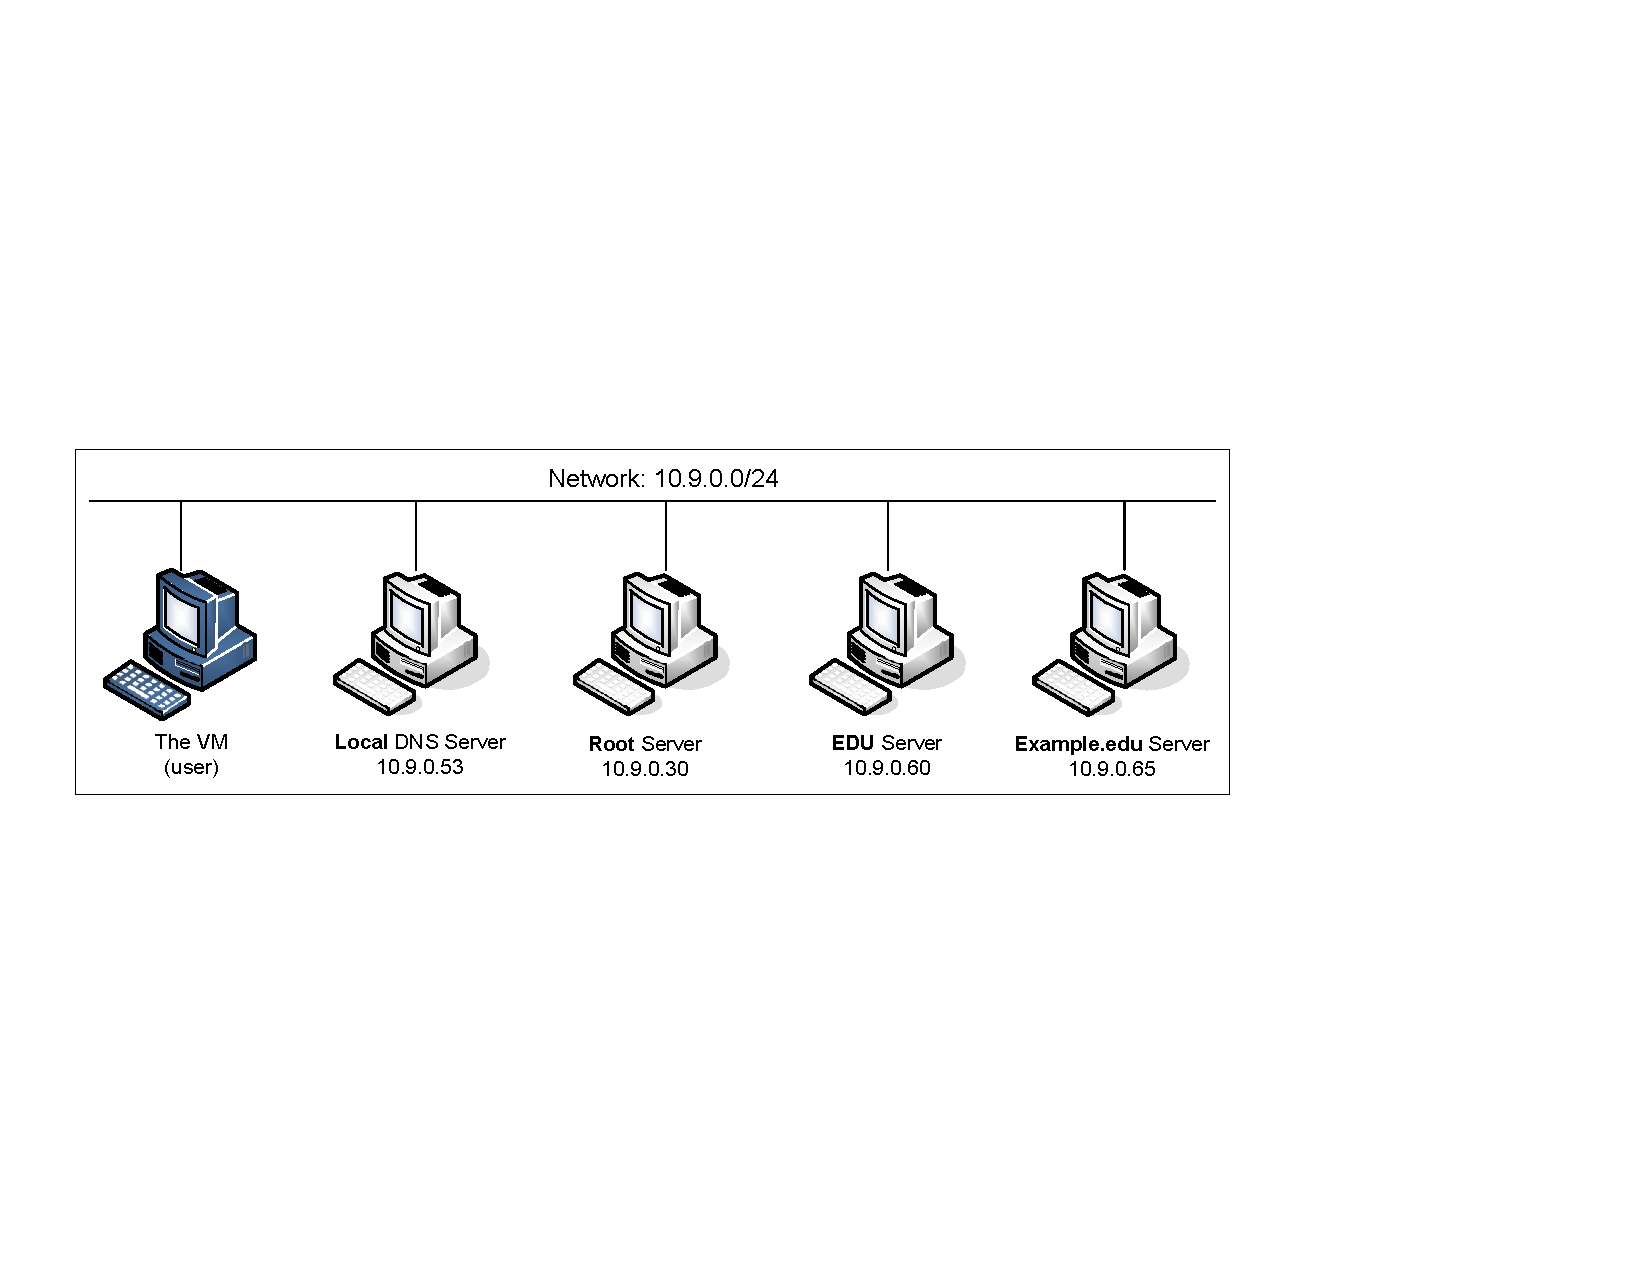
\includegraphics[width=0.95\textwidth]{Figs/DNS-in-a-box.pdf}
\end{center}
\caption{A simplified DNS infrastructure}
\label{dns:fig:dns-in-a-box}
\end{figure}


In this task, we will build a simplified DNS infrastructure, which 
consists of four nameservers, each one representing 
a specific role in the entire DNS infrastructure. 
In the real world, these nameservers are on different 
networks, but in this lab, for the sake of simplicity, we place them
on the same network. Figure~\ref{dns:fig:dns-in-a-box} depicts the system setup. 
Our DNS system includes the following nameservers: 

\begin{itemize}[nosep]
\item Local DNS server: conduct the DNS resolution process for other computers.
\item Root server: a nameserver serving the root zone.
\item \texttt{edu} server: nameserver serving the \texttt{edu} zone, a Top Level Domain (TLD).  
\item \texttt{example.edu} server: nameserver serving the \texttt{example.edu} zone. 
\end{itemize}




In this task, we will build a container for each name server separately. In the next
task, we will integrate them together to form a miniature DNS infrastructure. 
 


% -------------------------------------------
% SUBSECTION
% ------------------------------------------- 
\subsection{Task 2.a: Building the nameserver for \texttt{example.edu}}

In this task, we will build a nameserver for a domain 
called \texttt{example.edu}. We will build a container 
for this nameserver. First, we need to create a new folder to
store all the files necessary for building the container.
We will copy all the files from Task 1 to this folder, and these files serve
as the base for our new container. We will make changes to this base image. 


\paragraph{Step 1. Adding the zone entry}. We will 
add the following zone entry to the 
\path{named.conf} file. This entry indicates that the current nameserver 
is the master server for this domain, and the zone file is 
specified in the \texttt{file} entry.  


\begin{lstlisting}
zone "example.edu" {
        type master;
        file "/etc/bind/example.edu.db";
};
\end{lstlisting}


\paragraph{Step 2. Creating the zone file}. We will 
create a zone file called \texttt{example.edu.db} 
in the current folder, and then add the following
\texttt{COPY} command to the \dockerfile. It should be 
noted that in Task 1, we have already added a few 
\texttt{COPY} entries to the \dockerfile, so make sure they 
stay there. 


\begin{lstlisting}
COPY example.edu.db       /etc/bind/
\end{lstlisting}


Students should create their own zone file. An example
zone file is provided in the following. Most of the IP 
addresses in this zone file can be fake for the lab tasks, except 
the one for \texttt{ns.example.edu}, which needs to
be the real IP address of the container. 
In this example, we use \texttt{172.20.0.65} as the IP
address for the container.


\begin{lstlisting}
$TTL 3D
@       IN      SOA   ns.example.edu. admin.example.edu. (
                2008111001
                8H
                2H
                4W
                1D)

@       IN      NS    ns.example.edu.

@       IN      A     1.2.3.4
www     IN      A     1.2.3.5
ns      IN      A     172.20.0.65
*       IN      A     1.2.3.6
\end{lstlisting}
 
 


\paragraph{Step 3. Testing.} Follow the instruction in Task 1 
to build and start the container. Once the container is running,
run the following command from your VM (i.e., outside of the 
container). You need to replace the IP address in the 
command with the actual IP address of your container. If your 
setup is successful, you can get the IP address specified
in your zone file. 

\begin{lstlisting}
$ dig @172.20.0.65 example.edu
... 
;; ANSWER SECTION:
www.example.edu.    259200   IN  A   (*@\textbf{1.2.3.5}@*)
...
\end{lstlisting}




% -------------------------------------------
% SUBSECTION
% ------------------------------------------- 
\subsection{Task 2.b: Building the \texttt{edu} TLD server}

In this task, we will build a nameserver for a TLD domain, 
the \texttt{edu} domain.
Just like Task 2.a, we will
create a new folder for this container, and copy all the 
files from the base containers created in Task 1. 

%
%Note: try to avoid using \texttt{com} and \texttt{net}. It 
%is harder, because they depend on each other.

\paragraph{Step 1. Adding the zone entry}. We will
add the following zone entry to the
\path{named.conf} file. This entry indicates that the current nameserver
is the master server for this domain, and the zone file is
specified in the \texttt{file} entry.


\begin{lstlisting}
zone "edu" {
        type master;
        file "/etc/bind/edu.db";
};
\end{lstlisting}


\paragraph{Step 2. Creating the zone file}. We will
create a zone file called \texttt{edu.db}
in the current folder, and then add a corresponding
entry in the \dockerfile to copy \texttt{edu.db}
to the container. 


In this zone file, we will use the 
nameserver container developed in the previous task as the nameserver
for the \texttt{example.edu} domain. To achieve that,
we need to add an \texttt{NS} record and an {A} record 
in the zone file. This way, when a client ask us for
anything inside the \texttt{example.edu} domain, we can
tell them the nameserver (and its IP address) for this domain. 
See the following example.


\begin{lstlisting}
$TTL 3600
@       IN      SOA   a.tld-edu-servers.edu. admin.tld-edu-servers.edu. (
                2008111001
                8H
                2H
                4W
                1D)

@       IN      NS    a.tld-edu-servers.edu.

a.tld-edu-servers.edu.	IN 	A	172.20.0.60

example.edu.		IN	NS	ns.example.edu.
ns.example.edu.		IN	A	172.17.0.65

syr.edu.                IN      NS      ns1.syr.edu.
ns1.syr.edu.            IN      A       128.230.12.8
\end{lstlisting}


In addition to the record of the \texttt{example.edu}, please add at least 
three real domain names to this zone file. You can find their real
nameservers using \texttt{"dig <name> NS"} (e.g., \texttt{"dig syr.edu NS"}). 
In the example above, I have added two records for the \texttt{syr.edu} 
domain. 


\paragraph{Step 3. Testing.}
Follow the instruction in Task 1
to build and start the container. Once the container is running,
run the following command from your VM (i.e., outside of the
container). You  need to replace the IP address in the
command with the actual IP address of your 
\texttt{edu} container. If your
setup is successful, you can get the IP address specified
in your zone file (I have assigned \texttt{172.20.0.60} as the 
IP address for this nameserver).

\begin{lstlisting}
$ dig @172.20.0.60 www.example.edu
...
;; AUTHORITY SECTION:
example.edu.		3600	IN	NS	ns.example.edu.

;; ADDITIONAL SECTION:
ns.example.edu.		3600	IN	A	(*@\textbf{172.20.0.65}@*)
...
\end{lstlisting}


Try some domain names (ended with \texttt{edu}) that are not 
specified in your zone file, and see what happens. 




% -------------------------------------------
% SUBSECTION
% ------------------------------------------- 
\subsection{Task 2.c: Building root server}

In this task, we will build a root nameserver, serving the 
root zone. The procedure is quite similar to building
the \texttt{edu} zone, so we will not repeat it.  


We will create a zone file called \texttt{root.db}. 
For every TLD zone that we would like to include in our 
miniature DNS system, we need to add at least two entries 
in the zone file, including an \texttt{NS} record 
and an \texttt{A} record.  In the following example,
we have added the nameserver information for the 
\texttt{com} zone (the data in both records are real data).
We have also added the nameserver information 
for the \texttt{edu} zone, but since we are 
hosting the \texttt{edu} nameserver ourselves, the 
information is based on our own setup.


\begin{lstlisting}
com.                    IN   NS  a.gtld-servers.net.
a.gtld-servers.net.     IN   A   192.5.6.30

edu.                    IN   NS  a.tld-edu-servers.edu.
a.tld-edu-servers.edu.  IN   A   172.20.0.60
\end{lstlisting}
 

You should include records for at least five different TLDs, including two
hosted by you and the others hosted in the real world. 



\paragraph{Testing.} 
Follow the instruction in Task 1 to build and start the container. 
In this description, we choose to assign the 
IP address \texttt{172.20.0.30} to root server container.
Once the container is running,
run the following \texttt{dig} commands from your VM.
You should provide evidences to show that your root server does support the 
five required TLDs.

\begin{lstlisting}
$ dig @172.20.0.30 www.example.edu
$ dig @172.20.0.30 www.example.com
\end{lstlisting}


% -------------------------------------------
% SUBSECTION
% ------------------------------------------- 
\subsection{Task 2.d: Building the Local DNS Server} 

When a computer needs to resolve the IP address from a hostname (or vice versa),
it sends a request to its helper, which is called local DNS server (it
does not need to be local).  This local DNS server will conduct the 
entire DNS resolution process, and then send the result back to the computer. 
In this task, we will set up this local DNS server. 


\paragraph{Step 1. Get the root hint file.}

If the local DNS server cannot find the answer from its cache, it 
will go through an iterative process to get the answer from outside 
nameservers.  The process starts from the root server. 
Therefore, the local DNS server needs to
know the IP address of the root servers. 


In \path{/etc/bind/named.conf.default-zones}, which is included 
in \bind's configuration file \path{/etc/bind/named.conf}, there is an 
entry for the root zone. This entry specifies a hint file for the
root zone, and that is how the local DNS server knows the IP address of the
root server. 


\begin{lstlisting}
zone "." {
	type hint;
	file "/usr/share/dns/root.hints";
};
\end{lstlisting}
 
The root hint file specifies the nameservers for the 
root zone (there are 13 nameservers for the root zone). The 
IP address (v4 and v6) for these nameservers are provided in this file. 
The following example shows a snippet of the file. 


\begin{lstlisting}
.                        3600000      NS    A.ROOT-SERVERS.NET.
A.ROOT-SERVERS.NET.      3600000      A     198.41.0.4
A.ROOT-SERVERS.NET.      3600000      AAAA  2001:503:ba3e::2:30
...
\end{lstlisting}


We will copy this file to our container folder, because we need to make changes
to this file for our container image. Add the 
following entry to the \dockerfile, so when the container is built, our 
modified file \texttt{root.hints} will be copied into the container
image. 


\begin{lstlisting}
COPY root.hints           /usr/share/dns/
\end{lstlisting}
 


\paragraph{Step 2. Starting the server.} We run the following commands
to build and start the local DNS server container.

\begin{lstlisting}
$ docker build -t dns_local_server .
$ docker run --net seednetwork --ip 172.20.0.20 --rm -it dns_local_server
\end{lstlisting}
 

\paragraph{Step 3. Testing.} Once the container is started, we can
send the following query to it. This time, we should get the actual IP address 
that is hosted in our \texttt{example.edu} zone. 

\begin{lstlisting}
$ dig @172.20.0.20 www.example.edu

...
;; ANSWER SECTION:
www.example.edu.	259165	IN	A	1.2.3.5
...
\end{lstlisting}



% -------------------------------------------
% SUBSECTION
% ------------------------------------------- 
\subsection{Task 2.e: Configure our VM to use this local DNS server} 

So far, we need to use \texttt{@<ip>} in our \texttt{dig} command
to indicate what DNS server the \texttt{dig} command should talk to. While this 
is not an issue for \texttt{dig}, it is a problem for other software that 
depends on DNS. We need to tell the operating system that the 
DNS server container built in this task is the system's 
local DNS server. 

This is achieved by changing
the resolver configuration file~(\texttt{/etc/resolv.conf}) of the user machine,
so the container's IP address is added as the first \texttt{nameserver} entry in the file, i.e.,
this server will be used as the primary DNS server.
Unfortunately, our provided VM uses the Dynamic Host Configuration Protocol (DHCP) to obtain
network configuration parameters, such as IP address, local DNS server, etc.
DHCP clients will overwrite the \texttt{/etc/resolv.conf} file with the information
provided by the DHCP server.

One way to get our information into \texttt{/etc/resolv.conf} without worrying about
the DHCP is to add the following entry to the \path{/etc/resolvconf/resolv.conf.d/head}
file:

\begin{lstlisting}
Add the following entry to /etc/resolvconf/resolv.conf.d/head
  nameserver 172.20.0.20

Run the following command for the change to take effect
$ sudo resolvconf -u
\end{lstlisting}

The content of the head file will be prepended to the dynamically generated resolver
configuration file. Normally, this is just a comment line (the comment in
\texttt{/etc/resolv.conf} comes from this head file).


After you finish configuring the user machine, repeat 
the testing commands in Task 2.d, but this time, do not 
include the \texttt{@<ip>} in the command. Pay attention to 
the highlighted IP address to check whether the response does 
come from your container. If the setup is unsuccessful,
the IP will be \texttt{127.0.0.53}. 

\begin{lstlisting}
$ dig abc.example.edu

...
;; ANSWER SECTION:
abc.example.edu.	259200	IN	A	1.2.3.6

;; Query time: 3 msec
;; SERVER: (*@\textbf{172.20.0.20}@*)#53(172.20.0.20)
...
\end{lstlisting}
 




% *******************************************
% SECTION
% ******************************************* 
\section{Task 3: System Integration}

In the previous task, we have been building our nameserver containers 
individually. As the number of 
nameservers increases, the process become tedious. Fortunately,
docker provides a tool called \texttt{Compose}, which 
is for defining and running multi-container Docker applications. 
With Compose, we use a YAML file to configure our containers. Then, with a single command, 
we can create and start all the containers from your configuration.

\paragraph{Step 1. Writing the \texttt{docker-compose.yml} file.}
In the \texttt{docker-compose.yml} file, we can use \texttt{services} to 
create individual containers, and use \texttt{networks} to 
create networks. The following example lists two 
service entries and one network entry. 

\begin{lstlisting}[caption={\texttt{docker-compose.yml}}]
version: '3'

services:
  local_server:                  
    build: ./local_server
    tty: true
    networks:
      mynetwork:
        ipv4_address: 172.20.0.20

  root_server:
    build: ./root_server
    tty: true
    networks:
      mynetwork:
        ipv4_address: 172.20.0.30

  ... other entries are omitted ...
   

networks:
    mynetwork:
      ipam:
        config:
        - subnet: 172.20.0.0/24
\end{lstlisting}

Let us use the first service entry to explain how it works. 

\begin{itemize}
\item \texttt{build: ./local\_server}: This entry indicate that the container's folder 
is \texttt{local\_server}, and will use the \texttt{Dockerfile} inside to build the container.

\item \texttt{tty: true}: Indicate that when running the container, use the 
\texttt{-t} option, which is necessary for getting a shell prompt 
on the container later on. 

\item \texttt{networks}: specify the name of the networks that this container is attached to,
and the IP address statically assigned to the container. You can attach multiple networks
to the container. 
\end{itemize}
 

\paragraph{Step 2. Starting the containers.}
We can use the following commands to build the containers first, and then 
use the \texttt{up} command to start all the containers. Once we are done,
we can use the \texttt{down} command to stop and delete all the running containers.  


\begin{lstlisting}
// Build the containers 
$ docker-compose build

// Start all the containers 
$ docker-compose up

// Stop all the containers
$ docker-compose down
\end{lstlisting}


\paragraph{Note 1: Network issues.}
Since we have created a network in Task 2, and that network
conflicts with the one used in the docker compose file. If we want to 
stick to the same IP address assignment, we can delete the existing 
network before running the \texttt{docker-compose} commands. 
Use the following commands to find and delete networks. 


\begin{lstlisting}
// List all the existing networks 
$ docker network ls 

// Remove a network
$ docker network rm <name of network>
\end{lstlisting}
 

\paragraph{Note 2: Running commands on a running container}.
When we use \texttt{docker-compose} to run the container, those 
containers will run in the background. 
Sometimes, we need to run additional commands on a running container.
To do that, we can use the following commands to first 
get a container's ID, and then use \texttt{"docker exec"} 
to start a shell. 


\begin{lstlisting}
// Find the container's ID 
$ docker ps 

$ docker exec -it <container ID> /bin/bash
#  -- you will get a root shell 
\end{lstlisting}
 



% *******************************************
% SECTION
% ******************************************* 
\section{Task 4: Making It More Realistic}


In this task, we will make our miniature DNS system
a little bit more realistic. 

% -------------------------------------------
% SUBSECTION
% ------------------------------------------- 
\subsection{Task 4.a: Hosting more nameservers}


\begin{itemize}
\item Adding 2 more root servers. The real-world DNS system has 13 different 
IP address for the root server. We will create 3 in this lab.

\item Hosting two TLD servers. One is \texttt{edu}, which is already 
done in Task 2. The other one is your choice. 
You can find all the existing TLD names from the 
real root zone file: \url{https://www.internic.net/domain/root.zone}.
You can pick one from there or come up with one yourself. 
It costs a lot to buy a new TLD name in the real world, but in this lab, you 
can ``own'' one for free. 

\item For each TLD, build a second-level domain, in
addition to \texttt{example.edu} that is already built in Task 2. 
Use your first name as the domain name. 
For example, if your first name is \texttt{Bob}, you need to build the containers 
for the \texttt{bob.edu} and \texttt{bob.<tld>} domains,
where \texttt{<tld>} is the name for a Top-Level Domain selected
by you. 
\end{itemize}
 




% -------------------------------------------
% SUBSECTION
% ------------------------------------------- 
\subsection{Task 4.b: Supporting more TLDs}


At least supporting the following: 
\texttt{com}, \texttt{net}, \texttt{org}, and 
a selected country-code TLD (ccTLD).

We will not host the nameservers for these TLD domain, but 
if a user query a hostnames in these domains using our miniature
DNS system, they should get correct answers.  

To achieve that, we just need to ``register'' these TLD nameservers
with our root servers. 
There are many ways to find out the nameserver for a TLD. For example,
you can use the real-world zone file; you can directly
get it using \texttt{dig}. By running \texttt{"dig com NS"}, you
can get a list of nameservers for the \texttt{com} domain.
You can then get the IP address for each nameserver. 




% -------------------------------------------
% SUBSECTION
% ------------------------------------------- 
\subsection{Task 4.c: Supporting other domain names in \texttt{edu}}


You should support at least five real-world domain names 
in the \texttt{edu} domain. For these domains, when you run
the \texttt{dig} command, you should get their real IP address. Your
DNS system should support this. You should not run 
the nameservers for these domains; instead, you should modify
your \texttt{edu} nameserver, so it can direct the client
to the corresponding nameservers. 


You can use the \texttt{"dig <domain> NS"} command to get the nameservers
for a specified domain. See the following example. 

\begin{lstlisting}
$ dig syr.edu NS 
;; ANSWER SECTION:
syr.edu.		900	IN	NS	ns1.syr.edu.
syr.edu.		900	IN	NS	ns2.syr.edu.
\end{lstlisting}
 

 





% *******************************************
% SECTION
% ******************************************* 
\section{Submission}

%%%%%%%%%%%%%%%%%%%%%%%%%%%%%%%%%%%%%%%%

You need to submit a detailed lab report, with screenshots,
to describe what you have done and what you have observed.
You also need to provide explanation
to the observations that are interesting or surprising.
Please also list the important code snippets followed by
explanation. Simply attaching code without any explanation will not
receive credits.

%%%%%%%%%%%%%%%%%%%%%%%%%%%%%%%%%%%%%%%%



\end{document}
